% Options for packages loaded elsewhere
\PassOptionsToPackage{unicode}{hyperref}
\PassOptionsToPackage{hyphens}{url}
%
\documentclass[
]{book}
\usepackage{amsmath,amssymb}
\usepackage{lmodern}
\usepackage{ifxetex,ifluatex}
\ifnum 0\ifxetex 1\fi\ifluatex 1\fi=0 % if pdftex
  \usepackage[T1]{fontenc}
  \usepackage[utf8]{inputenc}
  \usepackage{textcomp} % provide euro and other symbols
\else % if luatex or xetex
  \usepackage{unicode-math}
  \defaultfontfeatures{Scale=MatchLowercase}
  \defaultfontfeatures[\rmfamily]{Ligatures=TeX,Scale=1}
\fi
% Use upquote if available, for straight quotes in verbatim environments
\IfFileExists{upquote.sty}{\usepackage{upquote}}{}
\IfFileExists{microtype.sty}{% use microtype if available
  \usepackage[]{microtype}
  \UseMicrotypeSet[protrusion]{basicmath} % disable protrusion for tt fonts
}{}
\makeatletter
\@ifundefined{KOMAClassName}{% if non-KOMA class
  \IfFileExists{parskip.sty}{%
    \usepackage{parskip}
  }{% else
    \setlength{\parindent}{0pt}
    \setlength{\parskip}{6pt plus 2pt minus 1pt}}
}{% if KOMA class
  \KOMAoptions{parskip=half}}
\makeatother
\usepackage{xcolor}
\IfFileExists{xurl.sty}{\usepackage{xurl}}{} % add URL line breaks if available
\IfFileExists{bookmark.sty}{\usepackage{bookmark}}{\usepackage{hyperref}}
\hypersetup{
  pdftitle={Linear Algebra: An Intuitionist Approach},
  pdfauthor={Matt Pettis},
  hidelinks,
  pdfcreator={LaTeX via pandoc}}
\urlstyle{same} % disable monospaced font for URLs
\usepackage{longtable,booktabs,array}
\usepackage{calc} % for calculating minipage widths
% Correct order of tables after \paragraph or \subparagraph
\usepackage{etoolbox}
\makeatletter
\patchcmd\longtable{\par}{\if@noskipsec\mbox{}\fi\par}{}{}
\makeatother
% Allow footnotes in longtable head/foot
\IfFileExists{footnotehyper.sty}{\usepackage{footnotehyper}}{\usepackage{footnote}}
\makesavenoteenv{longtable}
\usepackage{graphicx}
\makeatletter
\def\maxwidth{\ifdim\Gin@nat@width>\linewidth\linewidth\else\Gin@nat@width\fi}
\def\maxheight{\ifdim\Gin@nat@height>\textheight\textheight\else\Gin@nat@height\fi}
\makeatother
% Scale images if necessary, so that they will not overflow the page
% margins by default, and it is still possible to overwrite the defaults
% using explicit options in \includegraphics[width, height, ...]{}
\setkeys{Gin}{width=\maxwidth,height=\maxheight,keepaspectratio}
% Set default figure placement to htbp
\makeatletter
\def\fps@figure{htbp}
\makeatother
\setlength{\emergencystretch}{3em} % prevent overfull lines
\providecommand{\tightlist}{%
  \setlength{\itemsep}{0pt}\setlength{\parskip}{0pt}}
\setcounter{secnumdepth}{5}
\usepackage{booktabs}
\usepackage{braket}
\usepackage{mathtools}
\usepackage{amsmath}
\ifluatex
  \usepackage{selnolig}  % disable illegal ligatures
\fi
\usepackage[]{natbib}
\bibliographystyle{plainnat}

\title{Linear Algebra: An Intuitionist Approach}
\author{Matt Pettis}
\date{2021-11-28}

\begin{document}
\maketitle

{
\setcounter{tocdepth}{1}
\tableofcontents
}
\hypertarget{preface}{%
\chapter{Preface}\label{preface}}

\begin{quote}
And you may ask yourself, ``What is that beautiful house?''

And you may ask yourself, ``Where does that highway go to?''

And you may ask yourself, ``Am I right? Am I wrong?''

And you may say to yourself, ``My God! What have I done?''

-- Talking Heads, ``Once in a Lifetime''
\end{quote}

\begin{quote}
What one fool can do, another can.

-- Ancient Simian Proverb

-- Sylvanus Thompson, ``Calculus Made Easy''
\end{quote}

\begin{quote}
``Everything is the way it is because it got that way.''

-- D'Arcy Wentworth Thompson
\end{quote}

I'd like to say I'm writing this ``for the democratization of science and math,'' but really, for my kids and their friends so that they don't get snookered into thinking this stuff is beyond them and therefore not for them. It is for you. It is everybody's birthright.

One of the best things about science, but one I've found least talked about in the classes that I took in high school and college, is the part that explains ``why do we think things work this way?'' Why do we believe things are made up of atoms? Why did people believe that without the ability to \emph{see} atoms? What is it about the technology we've built that confirms that things are made of atoms? We believe things like this because we concocted hypotheses and made experimental tests that ruthlessly and cumulatively. We make assumptions that are verifiably true, and then we reach a little further with logic and some more subtle observations, and extend the things we get to conclude, and what we have to throw away. That is a powerful process.

Somewhere along the way, math got divorced from that process. It wasn't helped by great mathematicians like Carl Gauss who called Number Theory ``the Queen of Mathematics'' mostly because it didn't have much in the way of application, and that was a good thing. Or the eminent mathematician G. H. Hardy, who said,

\begin{quote}
``I have never done anything''useful``. No discovery of mine has made, or is likely to make, directly or indirectly, for good or ill, the least difference to the amenity of the world.''
\end{quote}

The perspective was, and often is, that math is a thing more akin to art, like poetry, and though it is sometimes useful, its main value is in that it is beautiful and fun. Ironically, his favorite subject, number theory, is the foundation of our ability to transmit secrets safely on the internet, and does, in fact, probably cause more good and ill than he was comfortable with.

The downside of such a perspective is that it makes it seem like learning the discipline of mathematics is inscrutable. When you encounter mathematical definitions, such as, ``What makes a thing a vector space?'', or ``What makes a thing a group?'', or ``What makes a set measureable?'', what you read are a bunch of seemingly awkward little statements that seem either indecipherable, or unknowable, or so stupidly dead-simple as to make you wonder why one would even need to say such a thing. For instance, when we get to the definition of a vector space, you'll see this as a defining characteristic that your, uh, we'll call a thingy for now, needs to have to be called a vector space:

\[ (\vec{x} + \vec{y}) + \vec{z} = \vec{x} + (\vec{y} + \vec{z}) \]

For those familiar with how numbers work, this seems like something Captain Obvious would say about math. It could also make you wonder ``what's the point of saying such a thing?''

These definitions don't come in an inspiration, like Athena springing fully formed from the forehead of Zeus. When you study the history of mathematics, you'll see that when trying to come up with descriptions like this, mathematicians will often argue, and even disagree violently. You'll often see different characterizations like this depending on where you look, because originators disagreed on what was \emph{fundamental} about what was going on. For systems to be compatible, though, the fundamental assumptions of one camp need to be at least derivable from the other, and vice versa.

This monograph is intended give you the motivations of why linear algebra is the way it is. It will address:

\begin{itemize}
\tightlist
\item
  Where do those rules about a vector space come from?
\item
  What's the big deal about linear independence?
\item
  What would make you come up with an idea like an inner product?
\item
  What's helpful about orthogonality?
\item
  Eigenvectors: how do they even work?
\end{itemize}

I'll approach this as science would ideally approach this. What do we observe? What sort of simplifications can we make to help us understand what is going on? What sort of models help us understand the important parts?

\hypertarget{mathbbr2-pythagorean-theoroem-law-of-cosines-and-inner-products}{%
\chapter{\texorpdfstring{\(\mathbb{R}^2\), Pythagorean Theoroem, Law of Cosines, and Inner Products}{\textbackslash mathbb\{R\}\^{}2, Pythagorean Theoroem, Law of Cosines, and Inner Products}}\label{mathbbr2-pythagorean-theoroem-law-of-cosines-and-inner-products}}

\begin{quote}
It takes a very unusual mind to undertake the analysis of the obvious.

-- Alfred North Whitehead
\end{quote}

\begin{quote}
Point of view is worth 80 IQ points

-- Alan Kay
\end{quote}

\hypertarget{mathbbr2-the-pythagorean-theorem-and-the-law-of-cosines}{%
\section{\texorpdfstring{\(\mathbb{R}^2\), the Pythagorean Theorem, and the Law of Cosines}{\textbackslash mathbb\{R\}\^{}2, the Pythagorean Theorem, and the Law of Cosines}}\label{mathbbr2-the-pythagorean-theorem-and-the-law-of-cosines}}

Let's start with what we know pretty solidly -- the Pythagorean Theorem. We know that, if we have a triangle \(\triangle ABC\), with \(C\) being a right angle, then:

\[(\text{Pythagorean Theorem}) \ \ \ \ \ c^2 = a^2 + b^2\]

\begin{figure}

{\centering 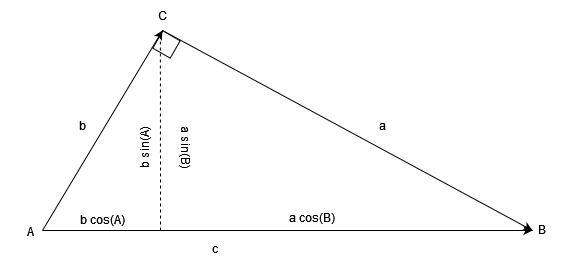
\includegraphics[width=0.75\linewidth,height=0.75\textheight]{images/LofC-PythThm} 

}

\caption{Pythagorean Theorem}\label{fig:unnamed-chunk-1}
\end{figure}

The thing to note here is that the relationship of the three sides in a right triangle has a very tidy little relationship according to the theorem. \(\vec{c}^2\) is totally determined by \(a\)'s and \(b\)'s value in a right triangle.

But what happens if we keep \(\vec{a}\) and \(\vec{b}\) the same length, but start to wiggle the right angle at the top, making it smaller or larger?

\begin{figure}

{\centering 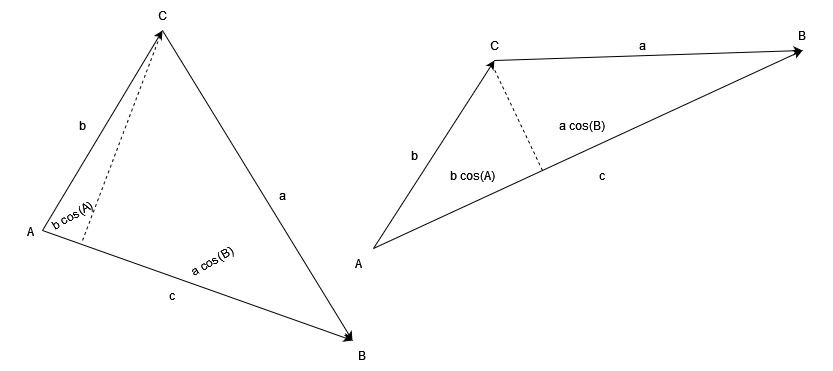
\includegraphics[width=0.75\linewidth,height=0.75\textheight]{images/LofC-acute-obtuse} 

}

\caption{Acute and obtuse triangles}\label{fig:unnamed-chunk-2}
\end{figure}

You'll note that the length of \(\vec{c}\) will shrink or grow from what it is in a right triangle with the same leg lengths. Can we make an equation like the Pythagorean Theorem that accounts for this deviation from what you get if you had a right triangle? Turns out, yes you can, and that \emph{adjusted} formula is known as \textbf{The Law of Cosines}:

\[(\text{Law of Cosines}) \ \ \ \ \ c^2 = a^2 + b^2 - 2 a b \ cos(C)\]

This should make some rough sense as a formula. As C shrinks below 90 degrees, the endpoints of the legs of the triangle get closer to each other, so the length of \(c\) shrinks. Algebraically, \(cos(C)\) becomes slightly positive, and \(-2 a b \ cos(C)\) will ultimately reduce the value of the right side of the equation, and \(c^2\) will be a little smaller than what it would be if \(C\) were a right triangle. In the other direction, as C grows above 90 degrees, the base of the triangle spreads, and \(c\) gets longer. Algebraically, \(cos(C)\) becomes slightly negative, and so \(-2 a b \ cos(C)\) becomes slightly positive, and \(c^2\) the right hand side makes \(c^2\) a little larger, so length \(c\) is a little larger.

I won't derive it here, as it is easy to find proofs. We should ask why this formula is important. Note that if you look at the diagrams, you will notice that:

\[(1) \ \ \ \ \ c = b \ cos(A) + a \ cos(B)\]

in all cases. That's pretty easy to see. What the Law of Cosines does, through some trigonometric identity substitutions, is re-express that equation, going from the angles that \(\vec{c}\) makes with \(\vec{a}\) and \(\vec{b}\), to using the angle that \(\vec{a}\) and \(\vec{b}\) make with each other instead. So the Law of cosines expresses \(\vec{c}\) totally in terms of the lengths of \(\vec{a}\) and \(\vec{b}\) and the angle they make with each other, never relying on information about \(c\).

It turns out that that this concept, of expressing vectors in terms of other vectors, is crucial in linear algebra, and we'll build up some concepts which may seem weird or abstract at the beginning, but turns out to be super useful in general, as it helps us lift off of reasoning about vector spaces in Euclidian space to general vector spaces.

\hypertarget{the-inner-product-or-dot-product}{%
\section{The Inner Product, or Dot Product}\label{the-inner-product-or-dot-product}}

Let's look at that adjustment factor to the Pythagorean Theorem that allows us to calculate any third side knowing the other two. Taking out the factor of \(-2\), we are left with:

\[(2) \ \ \ \ \ a b \ cos(C)\]

That particular computation, in Euclidian Space, is known as the \textbf{inner product of \(\vec{a}\) and \(\vec{b}\)}. It shows up in many contexts, and in general, the inner product will have different notations:
\[\vec{a} \cdot \vec{b}\]

\[ <\vec{a}, \vec{b}>\]

\[ <\vec{a}|\vec{b}>\]

How do we interpret this? There are a few components that go into building this up.

First is \(cos(C)\), which is the angle between \(\vec{a}\) and \(\vec{b}\). The cosine can be thought of as a measure of how much two lines, or vectors, point in the same direction. A value of 1 means they point completely in the same direction, -1 means they point in opposite directions, and 0 means that they are perpendicular to each other. We discussed above with the Law of Cosines that ``point-in-the-same-direction'' measure is baked into the adjustment to the Pythagorean Theorem to calculate the length of a third side of a triangle given the other two.

Second, how do we interpret multiplying the cosine by the lengths of \(a\) and \(b\)? Here we will make a stunning insight. Let's look back at equation (1). If we multiply both sides of the equation by \(c\), we get:

\[c^2 = cb\ cos(A) + ca\ cos(B)\]
or,
\[c^2 = \vec{c}\cdot\vec{b} + \vec{c}\cdot\vec{a}\]
by the definition of inner product we saw above. So if you squint, this kinda sorta looks like the Pythagorean Theorem. Furthermore, You can think of \(c^2\) as the inner product of a vector with itself, as the angle between a vector and itself can reasonably be thought of as 0, and \(cos(0) = 1\). So we can further rewrite the above as:

\[\vec{c}\cdot\vec{c} = \vec{c}\cdot\vec{b} + \vec{c}\cdot\vec{a}\]
Again, squinting, that is starting to look a lot like the Pythagorean Theorem, at least on the surface.

So, for Euclidian space, I like to think of the inner product, or dot product, as something you can calculate that accounts for how much in the same direction two vectors point (the cosine part), and add factors that make it dimensionally correct so that you can write a Pythagorean Theorem-like formula relating the lengths of sides of any triangle.

It turns out that the inner product has a lot of super-useful properties, mostly due to the high degree of symmetry it has.

What do I mean by ``symmetry''? Notice in the Pythagorean Theorem we distinguish between the hypotenuse and its legs. The formula only works when the square of the hypotenuse is on one side of the equation, and the squares of the legs are on the other side.

But this is not true of the Law of Cosines. The formula works no matter what two sides of the triangle you pick to derive the length of the third side from. That is, these formulas are all valid, and they have the same ``form'':

\[c^2 = a^2 + b^2 - 2 a b \ cos(C)\]
\[a^2 = c^2 + b^2 - 2 c b \ cos(A)\]
\[b^2 = a^2 + c^2 - 2 a c \ cos(B)\]

or,

\[\vec{c}\cdot\vec{c} = \vec{c}\cdot\vec{b} + \vec{c}\cdot\vec{a}\]
\[\vec{a}\cdot\vec{a} = \vec{a}\cdot\vec{b} + \vec{a}\cdot\vec{c}\]
\[\vec{b}\cdot\vec{b} = \vec{b}\cdot\vec{a} + \vec{b}\cdot\vec{c}\]

That's what I mean by symmetry, and that the Law of Cosines has it, but the Pythagorean Theorem does not.

\hypertarget{writing-vectors-in-terms-of-other-vectors}{%
\section{Writing vectors in terms of other vectors}\label{writing-vectors-in-terms-of-other-vectors}}

Apart from the nice observation that we can calculate lengths of a third side soley from information about the other two sides, who cares? We do. It turns out that a great simplification in dealing with vectors is if, instead of dealing with each vector on its own, like \(\vec{c}\) in \(\mathbb{R}^2\), we pick just two vectors that point in somewhat different directions, like \(\vec{a}\) and \(\vec{b}\), and then stretch or shrink those vectors (that is, make them point in the same direction, but of different lengths from the original), add them, and then use the sum of those two vectors as a stand-in for whatever vector \(\vec{c}\) we want. In math terms, we want to find multiples \(\alpha\) of \(\vec{a}\) and \(\beta\) of \(\vec{b}\) such that:

\[\vec{c} = \alpha\vec{a} + \beta\vec{b}\]
It may seem weird, but it does turn out that writing every possible vector \(\vec{c}\) in terms of two other vectors you pick at the outset (scalar multiples of \(\vec{a}\) and \(\vec{b}\)) makes other calculations you want to much more manageable. In the end, if you have some experience, you will probably end up picking \(\vec{a}\) and \(\vec{b}\) as you standard coordinate axes in the \(x\) and \(y\) direction, also denoted as either \(\hat{i}\) and \(\hat{j}\), or once you get into more dimensions than two, \(\hat{e}_{1}\) and \(\hat{e}_{2}\). But that will come later.

How do you do this? It turns out that you can calculate \(\alpha\) and \(\beta\) for that representation above purely with inner products, and combining inner products with the standard addition, subtraction, multiplication, and division operations. It's not pretty -- in fact, it looks kind of gross, but it is ultimately calculable. I won't go into the derivations of how you get there, but it turns out that with enough algebra, you can show that you can calculate the following. Mind you, don't look at the equations here right now and try to figure out how the terms are being used -- just note that you can indeed calculate the coefficients \(\alpha\) and \(\beta\) with just inner products and basic operations on numbers (add/subtract/multiply/divide). So, squint when you look at these equations:

\[\alpha = \frac{(\vec{a}\cdot\vec{b})\cdot(\vec{b}\cdot\vec{c})-(\vec{b}\cdot\vec{b})\cdot(\vec{a}\cdot\vec{c})}{(\vec{a}\cdot\vec{b})^2 - (\vec{a}\cdot\vec{a})\cdot(\vec{b}\cdot\vec{b})}\]
\[\beta = \frac{(\vec{a}\cdot\vec{b})\cdot(\vec{a}\cdot\vec{c})-(\vec{a}\cdot\vec{a})\cdot(\vec{b}\cdot\vec{c})}{(\vec{a}\cdot\vec{b})^2 - (\vec{a}\cdot\vec{a})\cdot(\vec{b}\cdot\vec{b})}\]
As I said, not the prettiest thing, but computable! And that is the goal. It may seem harder, but know that it is indeed far easier to pick a set of vectors and do these computations to represent them than it is to not have that.

\hypertarget{orthogonality-and-normality}{%
\section{Orthogonality and Normality}\label{orthogonality-and-normality}}

Those calculations are indeed a bit gross, so people have looked for ways to make that not so gross. Above we noted that when the angle between vectors is 90 degrees, the cosine is 0. That means that if the angle between \(\vec{a}\) and \(\vec{b}\) is 90 degrees, then \(\vec{a}\cdot\vec{b} = 0\). If you, at the outset, \emph{pick} the vectors \(\vec{a}\) and \(\vec{b}\) to be ones where the angle between them is 90 degrees, then the above calculations simplify greatly to:

\[\alpha = \frac{\vec{a}\cdot\vec{c}}{\vec{a}\cdot\vec{a}}\]

\[\beta = \frac{\vec{b}\cdot\vec{c}}{\vec{b}\cdot\vec{b}}\]
With this simplification, you should think, ``Wow, I should probably choose my vectors to be perpendicular to each other!'' And that is what orthogonality is -- vectors whose inner products are 0. When they are geometric vectors, like above, orthogonality is a synonym for perpendicularity. We just use \emph{orthogonality} in the future when we have inner product, but not good geometry to go with them.

To go one step further, as the dot product of a vector with itself is the square of the length of that vector, you can get even simpler expressions above if the length of \(\vec{a}\) and \(\vec{b}\) are \(= 1\). Then you can forget about the denomiators, as you then get:

\[\alpha = \vec{a}\cdot\vec{c}\]
\[\beta = \vec{b}\cdot\vec{c}\]
Having length one also has a general name, called being \emph{normal}, or \emph{normality}. And it too helps simplify calculations, like above. You can always compute a vector that is normal and in the same direction as your original vector if you divide the vector by its length. Or, scalar multiply it by its reciprocal length. So, for any vector \(\vec{v}\), regardless of length (other than 0), the following vector will have length 1:
\[\frac{1}{\sqrt{\vec{v}\cdot\vec{v}}}\cdot\vec{v}\]
Again -- same direction as \(\vec{v}\), but of length 1.

\hypertarget{gram-schmidt-orthonormalization}{%
\subsection{Gram-Schmidt Orthonormalization}\label{gram-schmidt-orthonormalization}}

Big words, straightforward idea.

Often, starting vectors for a given problem just kind of fall into your lap, and they are not orthogonal at the start. So how do we actually make an orthonormal set from one that isn't? Luckily, if you can use those starting vectors (that are not orthogonal) to make all of the other vectors you want, like above, you can can calculate a new set of vectors that will do the same thing, \emph{and} those vectors will be orthonormal. Here is a picture -- note the algebra looks worse than it is.

\begin{figure}

{\centering 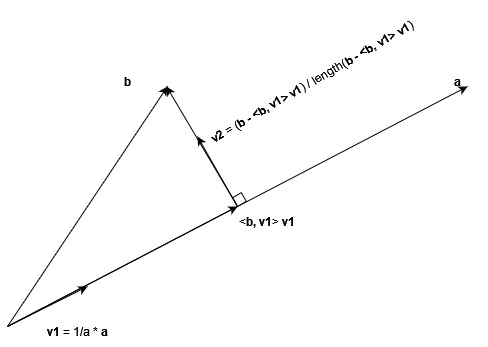
\includegraphics[width=0.75\linewidth,height=0.75\textheight]{images/gram-schmidt} 

}

\caption{Gram-Schmidt: algebra looks worse than it is.}\label{fig:unnamed-chunk-3}
\end{figure}

Here's the idea, in straightforward language.

\begin{itemize}
\tightlist
\item
  Take your two vectors, \(\vec{a}\) and \(\vec{b}\), and pick one of them to start. Say, \(\vec{a}\).
\item
  Normalize it by dividing by it's length, and call the result \(v1\). Congrats, you have your first orthonormal vector of your new set.
\item
  Find the spot/vector along \(\vec{v1}\), which is the same line/direction as \(\vec{a}\), that will make a right triangle with \(\vec{b}\). Turns out, this calculation is straightforward, and is \(<\vec{b},\vec{v1}>\ \vec{v1}\), or \((\vec{b}\cdot\vec{v1})\ \vec{v1}\).
\item
  Subtract that from \(\vec{b}\), which is \(\vec{b} - (\vec{b}\cdot\vec{v1})\ \vec{v1}\). What you are left with is a vector perpendicular to \(\vec{v1}\), so you are almost home.
\item
  Divide that vector by its own length so that you have a normalized vector: \(\vec{v2} = \frac{1}{length(\vec{b} - (\vec{b}\cdot\vec{v1})\ \vec{v1})}\ (\vec{b} - (\vec{b}\cdot\vec{v1})\ \vec{v1})\). Not as ugly as it seems. Congrats, you now have an orthonormal basis with \(\vec{v1}\) and \(\vec{v2}\).
\end{itemize}

This process can be extended to more than 2 dimensions. It is a process of taking vectors, scaling them to length 1 for normalization, finding projections (making right triangles and picking the cosine leg), subtracting it from your next vector, and then normalizing again. It's like a great big geometric construction you might have done in geometry in high school with a compass and straight-edge. The process gets a little more algorithmically hairy for more dimensions, but it is repeating this same idea/process over and over again.

We will call the set of vectors that you can use to represent any other vector (with scalar multiplication and addition) as a \emph{basis}. If all of the vectors in that basis are of length 1 and are perpendicular, we call that an \emph{orthonormal basis}.

\hypertarget{summarizing-the-big-points}{%
\section{Summarizing the big points}\label{summarizing-the-big-points}}

We've only worked with \(\mathbb{R}^2\), but we've learned a lot and scaffolded ourselves to work with some more abstract ideas. They are:

\begin{itemize}
\tightlist
\item
  You can generalize the Pythagorean Theorem via the Law of Cosines. This allows you to compute the length of any leg of a triangle from the length of the other two sides and the angle between the other two sides.
\item
  The Law of Cosines has embedded in it a quantity we end up calling the \emph{inner product} of two vectors. This gives some measure of how much in the same direction two sides of a triangle point, and incorporate the length of those two sides so that ultimately you can get a Pythagorean Theorem like equation.
\item
  The inner product has a lot of symmetries that allow you to flexibly compute any of the sides.
\item
  If we pick the right vectors, we can use the inner product, and standard addition/subtraction/multiplication/division to compute coefficients that can be used with those vectors to represent any other vector we want.
\item
  It's easier if the vectors we use to write other vectors with are mutually perpendicular and of length 1 (orthonormal).
\item
  We can always make an orthonormal set using the Gram-Schmidt process.
\end{itemize}

\hypertarget{a-closer-look-at-inner-products}{%
\chapter{A Closer Look at Inner Products}\label{a-closer-look-at-inner-products}}

To review, we used geometry and trigonometry to calculate the length of a side of a triangle in terms of the other two sides and the angle between those other two sides. This linked the Pythagorean Theorem to the Law of Cosines. Next, we showed that the quantity known as the \emph{inner product} was involved in these computations. Further, we could express any vector in terms of two other vectors that were both scaled appropriately and then added together. The scaling values we use can be calculated using just the inner product and basic arithmetic operations.

\hypertarget{how-do-i-work-this}{%
\chapter{How do I work this?}\label{how-do-i-work-this}}

My uncle tells the story of how they help transition mechanical engineers fresh out of school to working in industry. A senior engineer tasks them with a simple task: a near complete machine needs a piece -- it is missing a cog. The tell the new engineer to get them one. The new engineer studies the plans, designs the cog, painstakingly laying out the CAD designs for it, and comes back to the senior engineer after a week with his work to review how to machine that part, and how much it will cost. The senior engineer looks it over, says it is the right piece, and pulls out a catalog, and shows him how much it will cost to buy, usually at a fraction of the cost. The lesson they learn: don't create from scratch stuff you can buy cheaply from a catalog.

We might think of physics and mathematics having a similar relationship. Often, as you painstakingly observe a physical system, you figure out what are the important bits you need to capture with a model, and how those bits behave in the system. Then, you go shopping to your local math department, describing what you are doing, and hope that a mathematician can recommend a system they've already investigated that you can map your problem into, and take advantage of the notions, the notations, and theorems about the system behavior that they've already come up with.

So, let's proceed by looking at a simple spin-\(1/2\) system, of electrons that can have either a spin up or down measurement, depending on how the spin-detector is oriented. Many newer books start their quantum discussion this way, and two I can recommend that do this are \emph{Quantum Mechanics: The Theoretical Minimum} by Len Susskind and \emph{Quantum Mechanics: A Paradigms Approach} by David McIntyre. I won't repeat their treatment here, and will assume you know the basics of measuring spins in those systems. I will talk about how you start to pick your mathematics from the catalog to model this phenomenon.

\hypertarget{lay-of-the-land}{%
\section{Lay of the Land}\label{lay-of-the-land}}

Here is a picture that captures some of the important information about a quantum experiment we run:

\begin{figure}

{\centering 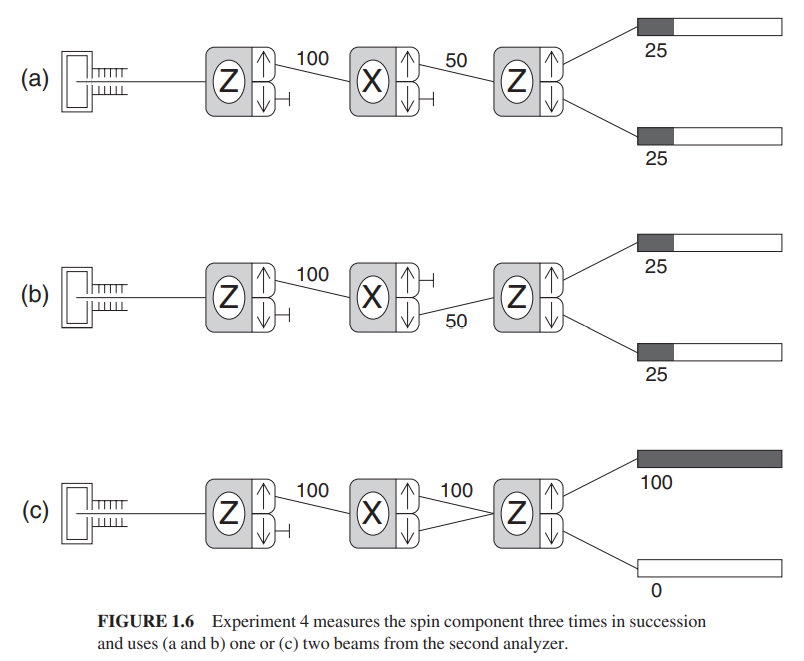
\includegraphics[width=0.75\linewidth,height=0.75\textheight]{images/McIntyre_two-spin-experiment} 

}

\caption{Two-spin experiment, McIntire}\label{fig:unnamed-chunk-11}
\end{figure}

Some notes on the picture:

\begin{itemize}
\tightlist
\item
  The apparatus on the left emits electrons, which have a spin we want to measure.
\item
  The detectors are labeled with a `Z' or `X' to tell you which direction in space we are orienting the detector. We pick the directions arbitrarily, but `Z' and `X' are orthogonal directions.
\item
  The arrows on the detectors indicate which spin orientation an electron comes out of. If it is measured with a spin up, relative to the how the detector is oriented, it exits from the top port, with the up arrow. If down, it exits from the lower port.
\item
  The labels \texttt{\textbar{}+\textgreater{}} and \texttt{\textbar{}-\textgreater{}} are also labels for the spins. The indicate absolute directions of the spin (spin up or down in the Z direction), rather than the up and down arrows on the port, that indicate if the spin is up or down \emph{relative to the how the port is oriented}, in the `Z' or `X' direction.
\item
  The labels \texttt{\textbar{}+\textgreater{}}\_x and \texttt{\textbar{}-\textgreater{}}\_x represent the absolute spin up/down orientations, but for the X direction. Again, the detector can be reoriented, but if the electron has one of these labels, it is independent of how the detector is oriented.
\item
  The numbers and shaded bars represent a percentage of electrons that end up in that bucket or state over a large number of electrons entering the system. Like a histogram.
\end{itemize}

Here are some things you, the experimenter, observe about the system:

\begin{itemize}
\tightlist
\item
  In (a), if you measure the Z spin, then the X spin, then the second time you measure the Z spin, it will be 50-50 up/down.
\item
  In (b), it just tells you that the same thing happens, no matter if the secon measurement for X is up or down, like in experiment (a).
\item
  In (c), somthing really weird happens: If you put the X spin detector in the middle, but carefully recombine both beams, as if you didn't measure the X spin, then the Z spin will be as if you didn't measure X spin at all, and stays in the spin state you measured it in in the first detector.
\end{itemize}

That can stand as the first of many weirdnesses you encounter in quantum. As McIntyre says: going from (a) or (b) to (c), it's as if you are in a half-lit room, throw open a window shade, and the whole room goes dark. In a classical model, (c) would still have a 50-50 split of spin measurements, but that doesn't happen in the quantum world.

\hypertarget{what-things-do-we-need-to-model-this}{%
\section{What things do we need to model this?}\label{what-things-do-we-need-to-model-this}}

So, we make the following observations.

\begin{itemize}
\tightlist
\item
  If we measure a spin as up in the Z direction, and keep measuring the spin with detectors all pointed along the same Z axis, we will always get the same spin up measurement. That is true as long as we don't orient the detector in a different direction.
\item
  Focusing on Z measurements, we have two states: spin up (\texttt{\textbar{}+\textgreater{}}) and spin down (\texttt{\textbar{}-\textgreater{}}). We get that with the detector registering a +1 or -1.
\item
  If we measure a Z spin with a detector, and it registers a +1, we call it spin up, and take a second, identical detector, and flip it upside, it will register a -1. This scenario is not pictured.
\item
  If we take a Z detector and measure a spin up electron, and then take a second detector, and start to slightly tilt the detector away from a straight Z orientation, we still only measure +1 and -1 readings. For a slight tilt, almost all electrons will measure spin up, and a few spin down. As it rotates to be perpendicular to the Z direction, electrons measure +1 and -1 with a 50\% probability. As we get closer to the tilt making the detector upside down, then most of the electrons will measure -1, until it is exactly upside down, and the detetcor will consistently measure -1.
\end{itemize}

This is kind of weird. Note that if this were a classical spin, you would expect that if you measured a spin of +1, and tilted the detector a little bit, you would measure a value a little less than +1. But quantum doesn't work that way. Instead of reducing the spin a little bit, what happens is that the probability of a +1 starts to decrease as you tilt the detector. The \emph{average} of multiple measurements approaches the value of what you would expect a single measured spin to decrease by (if it were classical).

So, whatever math we come up, it can't be the same classical math that gives a single spin measurement decreasing continuously from +1. It has to be something that accounts for:

\begin{itemize}
\tightlist
\item
  A spin will always either be +1 or -1
\item
  The \emph{probability} of detecting +1 and -1 change as you tilt the detector.
\end{itemize}

So we go talk to the math department\ldots{}

  \bibliography{book.bib,packages.bib}

\end{document}
